\section{Evidence from thinner books}\label{sec:thin}

The deepest book in crypto is the least likely place to find amplification. This section moves to thinner books. It reports the pre-registered out-of-sample tests in thin Binance books, on Bybit and in thin US stocks, failures included, and labels every check decided after a test set was opened as post hoc. Figure~\ref{fig:forest} collects all out-of-sample evaluations of this section.

\subsection{Design}\label{sec:thin_design}
We fixed 30 Binance USD-M perpetuals from the quote-volume ranking of one training day (June 10, 2024) before computing any T6 statistic, spread from BTCUSDT to symbols with under \$5M daily volume. Data are sampled on the 10th and 24th of each month from January 2023 to September 2026 and pass the validation rules V1--V5 of Section~\ref{sec:depth}: 2{,}565 of 2{,}700 symbol-days are valid; of 7{,}486{,}444 snapshots, V3 drops 212{,}745 and V4 drops 161{,}280, and V1 and V2 drop none. Liquidity terciles are fixed on median training-period depth within 1\% of the mid. The thin tercile has \$0.22M--\$0.38M of depth within 1\%, the thick tercile \$0.97M--\$220M. Flow is divided by each symbol's median absolute one-minute training flow, so that $\hat\kappa$ is in basis points per typical minute of flow. All other definitions follow Section~\ref{sec:depth}. An audit that scrambles all data from $t$ onward left every hourly feature unchanged in 30 of 30 trials.

\subsection{The cross-section of the amplification condition}

\begin{table}[t]\centering
\begin{threeparttable}
\caption{T6 estimates by liquidity tercile, 30 USD-M perpetuals, training days 2023--2024}\label{tab:x3}
\small\setlength{\tabcolsep}{5pt}
\begin{tabular}{lccc}
\toprule
 & Thick & Mid & Thin\\
\midrule
Mean $\hat C_3$ & $-0.0297$ & $-0.0216$ & $-0.0324$\\
\quad 95\% CI & [$-0.0341$, $-0.0257$] & [$-0.0250$, $-0.0185$] & [$-0.0386$, $-0.0268$]\\
Share of symbol-days with $\hat C_3>0$ & 9.4\% & 15.2\% & 16.1\%\\
Median $\hat\varphi$ & 2.33 & 2.38 & 3.11\\
Median $\hat\varepsilon$ & $-0.0014$ & $-0.0006$ & $-0.0005$\\
Share with $\hat\varepsilon>0$ & 11.1\% & 24.4\% & 30.1\%\\
Mean feedback loop gain $\hat Q$ & 0.0091 & 0.0033 & 0.0016\\
\midrule
\multicolumn{4}{l}{Spearman correlation with log depth across the 30 symbols [95\% CI]}\\
\quad mean $\hat C_3$ & \multicolumn{3}{c}{$-0.001$ [$-0.37$, $0.38$]}\\
\quad share $\hat C_3>0$ & \multicolumn{3}{c}{$-0.59$ [$-0.81$, $-0.27$]}\\
\quad $\hat Q$ & \multicolumn{3}{c}{$+0.70$ [$0.41$, $0.87$]}\\
\bottomrule
\end{tabular}
\begin{tablenotes}\footnotesize\item 1{,}424 training symbol-days, ten symbols per tercile. CIs from a symbol-day bootstrap (tercile rows) and a symbol bootstrap (correlations). $\hat Q$ is the loop gain of the companion paper estimated on one-minute bars; a placebo random walk with each day's volatility gives $\hat Q\approx0$ for every symbol. \end{tablenotes}
\end{threeparttable}
\end{table}

Table~\ref{tab:x3} confirms the BTCUSDT result across liquidity: mean $\hat C_3$ is negative in every tercile, and taker flow on average does not deplete the side it hits ($\hat\varepsilon<0$ at the median everywhere). What changes with depth is the frequency of the amplifying regime, not its average. The share of symbol-days with $\hat C_3>0$ rises from 9.4\% in the thick tercile to 16.1\% in the thin tercile, with a Spearman correlation of $-0.59$ against log depth. Depth sensitivity $\hat\varphi$ is larger, and depletion is less negative and more often positive, in thinner books. We had predicted a negative correlation between log depth and mean $\hat C_3$; that prediction fails ($\rho=-0.001$).

The last row is an unexpected finding for the companion paper. Measured feedback $\hat Q$ is larger in \emph{deeper} books ($\rho=+0.70$): flow responds to price deviations most where liquidity, and plausibly algorithmic participation, is greatest. Feedback and amplification are therefore different objects. Deep books have more feedback and refill fast enough to absorb it; thin books have less feedback and, more often, too little reversion.

\subsection{Overshoot and depletion}

\begin{table}[t]\centering\small
\begin{threeparttable}
\caption{Local-projection overshoot by tercile, $\max_{k\ge1}\beta_k-\beta_0$ [95\% CI]}\label{tab:x4}
\setlength{\tabcolsep}{3pt}
\begin{tabular}{lccc}
\toprule
 & Thick & Mid & Thin\\
\midrule
(A) total & $-0.045$ [$-0.079$, $0.047$] & $-0.034$ [$-0.054$, $0.024$] & $+0.007$ [$-0.050$, $0.083$]\\
(B) future flow fixed & $-0.181$ [$-0.211$, $-0.152$] & $-0.075$ [$-0.091$, $-0.058$] & $-0.073$ [$-0.094$, $-0.051$]\\
(C) flow and depth fixed & $-0.243$ [$-0.276$, $-0.212$] & $-0.121$ [$-0.140$, $-0.102$] & $-0.113$ [$-0.135$, $-0.092$]\\
Symbol-days & 459 & 460 & 445\\
\bottomrule
\end{tabular}
\begin{tablenotes}\footnotesize\item Basis points per typical minute of flow, horizons 0--30 minutes; local projections are estimated per symbol-day and averaged, with a symbol-day bootstrap. \end{tablenotes}
\end{threeparttable}
\end{table}

With future flow held fixed there is no overshoot in any tercile (Table~\ref{tab:x4}); the registered prediction of a positive (B) overshoot in thin books fails. The response decays less in thin than in thick books, and holding depth fixed again makes it decay faster, as in Table~\ref{tab:d4}.

To check that replenishment is not an artefact of one-minute aggregation, we sum signed taker flow exactly between consecutive depth snapshots from trade-level data and estimate depletion $\varepsilon_{30}$ at about 30 seconds, with an additional coefficient on sweeps (intervals in the top decile of absolute flow). Table~\ref{tab:x8} reports five symbols on six training days each.

\begin{table}[t]\centering\small
\begin{threeparttable}
\caption{Depletion at the snapshot scale (about 30 seconds)}\label{tab:x8}
\setlength{\tabcolsep}{2.5pt}
\begin{tabular}{llcccc}
\toprule
Symbol & Tercile & $\hat\varepsilon_{30}$ [95\% CI] & Sweep extra [95\% CI] & $\hat\varepsilon$, 1 minute & Days $\hat\varepsilon_{30}>0$\\
\midrule
BTCUSDT & thick & $-0.0045$ [$-0.0058$, $-0.0033$] & $+0.0034$ [$0.0023$, $0.0046$] & $-0.0025$ & 0 of 6\\
XMRUSDT & mid & $-0.0042$ [$-0.0058$, $-0.0029$] & $+0.0037$ [$0.0025$, $0.0051$] & $-0.0011$ & 0 of 6\\
RLCUSDT & thin & $-0.0034$ [$-0.0065$, $-0.0012$] & $+0.0029$ [$0.0011$, $0.0058$] & $-0.0003$ & 1 of 6\\
CELRUSDT & thin & $-0.0015$ [$-0.0032$, $0.0001$] & $+0.0017$ [$0.0004$, $0.0031$] & $-0.0004$ & 2 of 6\\
CVXUSDT & thin & $+0.0010$ [$-0.0033$, $0.0060$] & $-0.0003$ [$-0.0040$, $0.0027$] & $+0.0004$ & 2 of 6\\
\bottomrule
\end{tabular}
\begin{tablenotes}\footnotesize\item Day bootstrap over six training days per symbol. Depth is measured in bands of $\pm1\%$ around the current mid, so a price move also recenters the band; this biases $\hat\varepsilon_{30}$ in an unknown direction. \end{tablenotes}
\end{threeparttable}
\end{table}

In these re-centred bands, replenishment is stronger, not weaker, at 30 seconds: $\hat\varepsilon_{30}$ is negative with a CI below zero in three of five symbols and is never significantly positive. Sweeps offset most of it, so a sweep leaves the hit side about as deep as before ($\hat\varepsilon_{30}$ plus the sweep coefficient lies between $-0.0012$ and $+0.0007$). On this measure, the depletion channel that drives Theorem~\ref{thm:peak}\ref{thm:t6} would be absent even in thin books; the next subsection shows that the measure itself is biased toward replenishment.

\subsection{Depletion on a fixed price grid}\label{sec:fixedgrid}
Binance's depth archive reports depth within bands around the \emph{current} mid. After a buy moves the mid up, the ask band shifts into deeper resting orders and the bid band away from resting bids, which mechanically makes the book look ask-heavy after a buy, the sign we estimate. Bybit's order-book files contain every level, so the band can be held fixed at the previous mid. After seeing Table~\ref{tab:x8} we computed, for the six coins of Table~\ref{tab:bybitob} on four days each, the change in depth imbalance over 30-second intervals regressed on signed taker flow, once with the band fixed at the start-of-interval mid and once re-centred at the end-of-interval mid, Binance's construction.

\begin{table}[t]\centering\small
\begin{threeparttable}
\caption{Depletion at 30 seconds with a fixed and a re-centred band (Bybit order books, post hoc)}\label{tab:fixedgrid}
\begin{tabular}{lccc}
\toprule
Band & $\hat\varepsilon_{30}$ [95\% CI] & Share $>0$ & Coin-days\\
\midrule
Fixed at previous mid & $+0.0021$ [$+0.0013$, $+0.0032$] & 95\% & 20\\
Re-centred (Binance) & $-0.0004$ [$-0.0007$, $-0.0001$] & 30\% & 20\\
\bottomrule
\end{tabular}
\begin{tablenotes}\footnotesize\item ACH, ALICE, API3, LIT, WOO and ZEN, May 11--12 and September 11--12, 2025; flow normalized by each coin-day's median absolute 30-second flow; mean over coin-days with a bootstrap interval. Post hoc. Kind: real data (Part 13, \texttt{R5}).\end{tablenotes}
\end{threeparttable}
\end{table}

The sign reverses (Table~\ref{tab:fixedgrid}). With the band fixed, buying depletes the ask side in 19 of 20 coin-days; with the band re-centred, the same data reproduce the replenishment of Tables~\ref{tab:d3} and~\ref{tab:x8}. The replenishment finding is therefore an artefact of band recentring, and depletion is present. Two conclusions survive. First, local projections show no peak overshoot once future flow is held fixed (Table~\ref{tab:x4}), so depletion is not large enough to satisfy $\varphi\varepsilon>(1-a)\kappa$ in the data we observe; second, the depth term carries no out-of-sample forecasting content (Tables~\ref{tab:y6} and~\ref{tab:z6}). Both statements rest on Binance's re-centred depth measure, and a fixed-grid measure of $\varphi\varepsilon$ in the same books would require order-level Binance data that are not public.

\subsection{Pre-registered test in thin books}\label{sec:x6}
Before opening 2025--2026 for these symbols we registered the specification (SHA-256 \texttt{5910b6b4d90a\ldots}). It is identical to Section~\ref{sec:depth} except for three changes, all fixed in advance: the primary sample is the thin tercile; the regressions include symbol fixed effects; and the bootstrap resamples dates, with all symbols on a date kept together. The test cell was executed twice in the same session. The specification hash, the code and the data were unchanged between the two runs, and the evaluation is deterministic, so both runs give the numbers below; we report the count because the protocol requires it.

\begin{table}[t]\centering
\begin{threeparttable}
\caption{Pre-registered test, 30 symbols, 2025--2026}\label{tab:x6}
\small\setlength{\tabcolsep}{4pt}
\begin{tabular}{llccc}
\toprule
Sample & Outcome $\mid$ candidate & $\Delta R^2$ (pts) [95\% CI] & $\Delta$AUC [95\% CI] & Holm $p$\\
\midrule
Thin (primary) & MAE $\mid\hat C_3$ & $+1.216$ [$+0.273$, $+7.987$] & $+0.012$ [$+0.003$, $+0.019$] & ---\\
Thin & MAE $\mid$ peak ratio & $+0.065$ [$-0.072$, $+0.108$] & $+0.000$ [$-0.000$, $+0.001$] & 0.207\\
Thin & depth collapse $\mid\hat C_3$ & $-2.111$ [$-3.127$, $-1.173$] & $-0.012$ [$-0.023$, $-0.003$] & 1.000\\
Thin & OI drop $\mid\hat C_3$ & $+0.184$ [$-0.242$, $+1.128$] & $+0.040$ [$+0.017$, $+0.061$] & $<0.001$\\
Mid & MAE $\mid\hat C_3$ & $+0.003$ [$-0.056$, $+0.875$] & $+0.002$ [$-0.002$, $+0.005$] & 0.551\\
Thick & MAE $\mid\hat C_3$ & $+0.039$ [$-0.244$, $+0.057$] & $-0.001$ [$-0.003$, $+0.000$] & 0.361\\
All 30 & MAE $\mid\hat C_3$ & $+0.117$ [$-0.015$, $+1.736$] & $+0.003$ [$-0.000$, $+0.006$] & $<0.001$\\
\bottomrule
\end{tabular}
\begin{tablenotes}\footnotesize\item Primary: train 8{,}340 and test 6{,}521 symbol-hours on ten symbols; Clark--West $t=8.53$, one-sided $p<0.001$; baseline out-of-sample $R^2=0.025$; AUC $0.768\to0.780$. The pre-registered test passes. Holm $p$ is the Clark--West $p$-value adjusted across the six secondary tests. Date-block bootstrap with 2{,}000 draws; bootstrap CIs are right-skewed because a few volatile dates carry much of the variation. \end{tablenotes}
\end{threeparttable}
\end{table}

The primary test passes (Table~\ref{tab:x6}). In thin books, $\hat C_3$ estimated from the previous six hours adds $1.2$ points of out-of-sample $R^2$ for the next hour's maximum adverse excursion, beyond realized volatility, flow, volume, depth, imbalance and open interest, and raises the AUC for tail hours by $0.012$. The effect is confined to thin books: in the mid and thick terciles it is zero, and in the pooled sample the Clark--West test rejects but the $\Delta R^2$ interval contains zero. $\hat C_3$ also helps classify hours with a large open-interest drop, but it predicts depth collapse \emph{worse} than the baseline, again pointing away from the depth channel.

\paragraph{Flags.} On training data we set a $\hat C_3$ flag and a volatility flag; 575 of 6{,}521 test hours (8.8\%) are tail hours. The $\hat C_3$ flag fires in 8.9\% of hours with precision 16.5\% and recall 16.7\%, about twice the base rate. The volatility flag, which fires more often (16.0\%), does better (precision 23.4\%, recall 42.4\%), and the union reaches recall 51.1\% at precision 19.5\%. $\hat C_3$ is a useful addition to volatility in thin books, not a replacement for it.

\subsection{Tick size: a caution and a robustness check}\label{sec:tick}

\paragraph{Tick changes.} We located tick changes by inferring each day's price grid and dating changes by binary search over daily files. We found 12 tick reductions, all by a factor of ten, on 11 symbols (GMTUSDT twice) between August 2023 and August 2026; nine fall in the test period. A difference-in-differences design compares 10 days before and after each event with four control symbols of similar liquidity. After a tick cut, $\hat C_3$ rises with a CI above zero in 10 of 12 events, but realized volatility in basis points falls sharply at the same time (by up to 32 bp on ALICEUSDT), and the implied peak ratio does not change in any event (every CI includes zero). The Spearman correlation between the change in refill $\hat r$ and the change in the peak ratio is $-0.04$. We read this as a measurement result, not a test of the theory: at a coarse tick, prices move in discrete steps and the basis-point scale of $\hat C_3$ changes mechanically when the grid changes. The natural experiment cannot test the prediction that faster refill lowers the overshoot.

\paragraph{Does tick size drive Table~\ref{tab:x6}?} Eleven of the 30 symbols, six of them thin, changed tick, and five of those six did so inside the test period. After seeing Table~\ref{tab:x6} we therefore ran the post-hoc checks of Table~\ref{tab:x6r}, counted separately (one evaluation).

\begin{table}[t]\centering\small
\begin{threeparttable}
\caption{Post-hoc tick-size robustness of the thin-book result}\label{tab:x6r}
\setlength{\tabcolsep}{3pt}
\begin{tabular}{p{0.34\textwidth}cccc}
\toprule
Check & Symbols & Test hours & $\Delta R^2$ (pts) [95\% CI] & Clark--West $p$\\
\midrule
R0 baseline (Table~\ref{tab:x6}) & 10 & 6{,}521 & $+1.216$ [$+0.295$, $+8.017$] & $<0.001$\\
R1 + relative tick size and its log & 10 & 6{,}485 & $+1.243$ [$+0.373$, $+7.627$] & $<0.001$\\
R2 drop symbols with any tick change & 4 & 2{,}639 & $+0.511$ [$-0.069$, $+2.061$] & $<0.001$\\
R3 only days with the training tick & 10 & 5{,}642 & $+1.131$ [$+0.256$, $+9.305$] & $<0.001$\\
R1 and R3 together & 10 & 5{,}642 & $+1.222$ [$+0.357$, $+9.410$] & $<0.001$\\
R4 outcome in ticks & 10 & 6{,}485 & $-0.127$ [$-0.319$, $-0.018$] & 0.991\\
R5 $\hat C_3$ percentile within symbol & 10 & 6{,}521 & $+0.158$ [$-0.013$, $+1.322$] & 0.026\\
R6 leave one symbol out (10 fits) & 9 & & $+0.698$ to $+1.760$, all CIs $>0$ & all $<0.001$\\
\bottomrule
\end{tabular}
\begin{tablenotes}\footnotesize\item Post hoc: decided after Table~\ref{tab:x6}. 500 date-block bootstrap draws (200 in R6). \end{tablenotes}
\end{threeparttable}
\end{table}

The result survives controls for tick size, the removal of every day traded at a tick different from training, and the removal of any single symbol (Table~\ref{tab:x6r}). It weakens when the six thin symbols that ever changed tick are dropped: four remain, and the point estimate halves with an interval that just includes zero. It disappears when the outcome is measured in ticks; at each tick cut this outcome jumps tenfold, a break the training fit cannot anticipate, so we regard R4 as a weak test, but we report it. A scale-free version of the candidate (its percentile within each symbol's training distribution) is weak. Our reading is that $\hat C_3$'s forecasting content is tied to its \emph{level}, which mixes the amplification balance with the basis-point scale of each book. Sections~\ref{sec:y6} and~\ref{sec:y8} test whether that level is more than a measure of scale.

\subsection{Out-of-sample replication on new symbols}\label{sec:y6}
A result found in ten symbols could be specific to them. We therefore drew 24 new symbols, seeded and before any analysis, from the 72 USD-M perpetuals that were not in the original 30 and whose training-day volume was at most 1.5 times that of the most liquid thin symbol. We applied the same validation (2{,}090 of 2{,}160 symbol-days valid) and classified symbols as thin with a cut fixed in advance at the boundary between the original thin and mid terciles (\$0.39M of depth within 1\%). Ten new symbols are thin (ACH, ARPA, CHR, GTC, HOT, IOTX, OGN, SPELL, T and ZEN, all USDT-margined) and 14 are not. A new specification (SHA-256 \texttt{6aa8e2c03d79\ldots}) fixed the primary test identical to Table~\ref{tab:x6} and, as secondary tests, the three terms of $C_3$ separately, a unit-free ratio $A=(\varphi\varepsilon+\kappa^2\eta q)/((1-a)\kappa)-1$ that is positive exactly when $C_3>0$, and the not-thin group. The test set was opened once.

\begin{table}[t]\centering
\begin{threeparttable}
\caption{Pre-registered replication on ten new thin symbols, 2025--2026}\label{tab:y6}
\small\setlength{\tabcolsep}{4pt}
\begin{tabular}{llccc}
\toprule
Sample & Candidate & $\Delta R^2$ (pts) [95\% CI] & $\Delta$AUC [95\% CI] & Holm $p$\\
\midrule
Thin (primary) & $\hat C_3$ & $+0.845$ [$+0.303$, $+6.371$] & $+0.008$ [$+0.002$, $+0.013$] & ---\\
Thin & momentum term $\kappa^2\eta q$ & $+0.641$ [$+0.395$, $+3.242$] & $+0.003$ [$-0.001$, $+0.008$] & $<0.001$\\
Thin & reversion term $(1-a)\kappa$ & $+0.688$ [$+0.204$, $+5.606$] & $+0.008$ [$+0.003$, $+0.012$] & $<0.001$\\
Thin & depth term $\varphi\varepsilon$ & $+0.013$ [$-0.213$, $+1.155$] & $-0.001$ [$-0.005$, $+0.003$] & 0.308\\
Thin & unit-free ratio $A$ & $-0.045$ [$-0.096$, $-0.031$] & $-0.000$ [$-0.001$, $+0.000$] & 0.974\\
Not thin (14) & $\hat C_3$ & $-0.042$ [$-0.131$, $+0.780$] & $+0.002$ [$-0.003$, $+0.007$] & 0.308\\
\bottomrule
\end{tabular}
\begin{tablenotes}\footnotesize\item Primary: train 8{,}520 and test 7{,}092 symbol-hours; Clark--West $t=11.66$, one-sided $p<0.001$; AUC $0.768\to0.776$; training coefficient $+54.3$ (Table~\ref{tab:x6}: $+88.3$). Training coefficients: momentum $+104.3$, reversion $-53.0$. The pre-registered replication passes. \end{tablenotes}
\end{threeparttable}
\end{table}

The result replicates (Table~\ref{tab:y6}). On symbols never used before, $\hat C_3$ adds $0.85$ points of out-of-sample $R^2$ with an interval excluding zero, and improves tail classification. It again has no value outside thin books. The decomposition shows where the forecasting content lies, and every sign matches Theorem~\ref{thm:peak}\ref{thm:t6} and Theorem~\ref{thm:peak}\ref{prop:t6m}. A larger momentum term predicts larger adverse excursions; a larger reversion term, which pushes $C_3$ down, predicts smaller ones; and the depth term, whose depletion factor is close to zero (Table~\ref{tab:x8}), predicts nothing. In training data the reversion term is by far the largest component (median $0.033$, against $-0.0009$ for momentum and $-0.0003$ for depth), so most of the variation in $\hat C_3$ is variation in impact-weighted mean reversion.

The unit-free ratio fails. Because the amplifying terms are small, its median is $-0.996$ and its variation is mostly the noise of a ratio with an estimated denominator. Together with R5 in Table~\ref{tab:x6r}, this means that on these samples the forecasting content was tied to the level of $\hat C_3$. Section~\ref{sec:z6} tests two better-behaved unit-free statistics on fresh data.

\subsection{Is $\hat C_3$ just price impact?}\label{sec:y8}
Both working terms contain the impact coefficient $\kappa$, so $\hat C_3$ might forecast excursions only because it measures illiquidity. After seeing Table~\ref{tab:y6} we added four impact controls, all from the same past six hours or hour and winsorized at training percentiles: $\hat\kappa$ from the same fit, $\hat\kappa^2$, a univariate Kyle's $\lambda$ \citep{kyle1985} (slope of returns on signed flow) and a log Amihud ratio \citep{amihud2002} (absolute return over volume). This is a post-hoc check, evaluated once and counted separately.

\begin{table}[t]\centering\small
\begin{threeparttable}
\caption{Post-hoc price-impact controls, ten new thin symbols, 2025--2026}\label{tab:y8}
\begin{tabular}{lccc}
\toprule
Candidate $\mid$ added controls & $\Delta R^2$ (pts) [95\% CI] & $\Delta$AUC [95\% CI] & Clark--West $t$\\
\midrule
$\hat C_3$ $\mid$ none (Table~\ref{tab:y6}) & $+0.845$ [$+0.303$, $+6.371$] & $+0.008$ [$+0.002$, $+0.013$] & 11.66\\
$\hat C_3$ $\mid$ $\hat\kappa$, $\hat\kappa^2$ & $+0.755$ [$+0.371$, $+4.718$] & $+0.006$ [$-0.000$, $+0.010$] & 6.63\\
$\hat C_3$ $\mid$ Kyle's $\lambda$, Amihud & $+1.089$ [$+0.498$, $+7.149$] & $+0.007$ [$+0.001$, $+0.013$] & 8.02\\
$\hat C_3$ $\mid$ all four & $+0.682$ [$+0.334$, $+4.525$] & $+0.004$ [$-0.001$, $+0.009$] & 5.69\\
Momentum term $\mid$ all four & $+0.487$ [$+0.311$, $+2.384$] & $+0.002$ [$-0.002$, $+0.006$] & 3.42\\
Reversion term $\mid$ all four & $+0.529$ [$+0.222$, $+3.762$] & $+0.005$ [$-0.000$, $+0.009$] & 8.45\\
$\hat\kappa$ alone $\mid$ none & $-0.026$ [$-0.084$, $+0.030$] & $+0.000$ [$-0.000$, $+0.000$] & $-1.77$\\
\bottomrule
\end{tabular}
\begin{tablenotes}\footnotesize\item Post hoc: decided after Table~\ref{tab:y6}. Same evaluation code and bootstrap as Table~\ref{tab:y6}; Holm-adjusted $p<0.001$ for every row except $\hat\kappa$ alone ($p=0.96$). Training correlations of $\hat C_3$ with the controls: $\hat\kappa$ $-0.43$, Kyle's $\lambda$ $-0.44$, Amihud $+0.10$. \end{tablenotes}
\end{threeparttable}
\end{table}

$\hat C_3$ is not a proxy for impact (Table~\ref{tab:y8}). With all four impact controls it keeps about 80\% of its gain in $R^2$ ($0.68$ of $0.85$ points), with an interval above zero, and both the momentum and the reversion terms survive separately. Impact on its own forecasts nothing. Controlling for Kyle's $\lambda$ and Amihud alone \emph{raises} the gain to $1.09$ points: once plain illiquidity is held fixed, the dynamic balance that $\hat C_3$ measures stands out more clearly. One qualification: with $\hat\kappa$ controlled, the gain in tail \emph{classification} is no longer significant. The robust claim is about the size of the next hour's adverse excursion, not about flagging tail hours beyond what impact already flags.

\subsection{A third test on fresh days}\label{sec:z6}
Parts 4 and 5 of the replication package use the 10th and 24th of each month. For a third test we registered a new specification (SHA-256 \texttt{65acda361861\ldots}) before downloading the 3rd and 17th of each month of 2025--2026, days never used in any analysis. Training reuses the 2023--2024 days of the earlier tests. The sample is all 20 thin symbols of Sections~\ref{sec:x6} and~\ref{sec:y6}, with the ten mid-tercile symbols as a negative control. Two changes make the test harder: the four price-impact controls of Table~\ref{tab:y8} are now part of the baseline, and because the specification has two primary hypotheses (this one and the backtest of Section~\ref{sec:backtest}) each is tested at $\alpha=0.025$ with 97.5\% intervals. The test set was opened once; 1{,}137 fresh symbol-days passed validation.

\begin{table}[t]\centering
\begin{threeparttable}
\caption{Pre-registered test on fresh days, 2025--2026 (impact controls in the baseline)}\label{tab:z6}
\small\setlength{\tabcolsep}{2.5pt}
\begin{tabular}{lp{0.27\textwidth}ccc}
\toprule
Sample & Candidate & $\Delta R^2$ (pts) [CI] & $\Delta$AUC [95\% CI] & Holm $p$\\
\midrule
Thin (primary) & $\hat C_3$ & $+1.583$ [$+0.588$, $+3.237$] & $+0.002$ [$-0.003$, $+0.006$] & ---\\
Thin & reversion term & $+1.442$ [$+0.679$, $+2.621$] & $+0.003$ [$-0.001$, $+0.006$] & $<0.001$\\
Thin & momentum term & $+0.422$ [$+0.000$, $+1.063$] & $-0.002$ [$-0.005$, $+0.001$] & $<0.001$\\
Thin & depth term & $+0.323$ [$+0.092$, $+0.639$] & $+0.001$ [$-0.001$, $+0.003$] & $<0.001$\\
Thin & gain multiple $S_{60}/|\hat h_0|$ & $+0.488$ [$+0.252$, $+0.851$] & $+0.000$ [$-0.001$, $+0.001$] & $<0.001$\\
Thin & log reversion half-life & $+0.619$ [$+0.351$, $+1.031$] & $+0.001$ [$+0.000$, $+0.003$] & $<0.001$\\
Thin & $\hat C_3$ without depth, $\hat C_3^{\rm flow}$ & $+1.747$ [$+0.725$, $+3.393$] & $+0.001$ [$-0.004$, $+0.006$] & $<0.001$\\
Mid (control) & $\hat C_3$ & $+0.055$ [$-0.047$, $+0.239$] & $+0.000$ [$-0.001$, $+0.001$] & 0.038\\
\bottomrule
\end{tabular}
\begin{tablenotes}\footnotesize\item Primary: train 16{,}860 and test 13{,}428 symbol-hours on 39 test dates; 97.5\% date-block bootstrap interval; Clark--West $t=9.46$, one-sided $p<0.001$; baseline out-of-sample $R^2=0.185$; training coefficient $+68.0$. The pre-registered test passes. Secondary rows: 95\% intervals, Holm-adjusted Clark--West $p$ across the eleven secondary tests of the specification. Thin: 20 symbols; mid: 10. The gain multiple and the half-life are unit-free. $S_{60}$ is the summed absolute impulse response over 60 minutes; $\hat C_3^{\rm flow}=\hat\kappa^2\hat\eta\hat q-(1-\hat a)\hat\kappa$ from the model without depth. \end{tablenotes}
\end{threeparttable}
\end{table}

The result holds a third time, and more strongly (Table~\ref{tab:z6}). On fresh days, with impact already in the baseline, $\hat C_3$ adds $1.6$ points of $R^2$ for the next hour's adverse excursion in thin books. Three findings sharpen the earlier picture. First, two unit-free statistics now work: the gain multiple, the summed response divided by impact, and the log half-life of reversion both add about half a point of $R^2$ with intervals above zero. The scale concern of Section~\ref{sec:tick} is therefore answered: the content is the dynamic balance, not the basis-point scale of the book, in the sense of the invariance hypotheses of \citet{kyle2016}. Second, the reversion term carries most of the signal, as Theorem~\ref{thm:sum} suggests, since $S$ depends on reversion through $1/(m-q\tilde\kappa)$. Third, the depth-free statistic forecasts as well as the full one, which matters for the next subsection. In mid-depth books the Clark--West test rejects at the Holm-adjusted 5\% level, but the $R^2$ gain is $0.06$ points with an interval that includes zero. As with the impact controls, the gain in tail \emph{classification} is not significant: the robust claim is about the size of excursions.

\subsection{Beyond volatility forecasting}\label{sec:z9}
The adverse excursion of the next hour is close to a volatility outcome, so a natural objection is that $\hat C_3$ only proxies for future volatility in a way the simple volatility controls miss. We registered a fourth test (SHA-256 \texttt{71983f1a9d2c\ldots}) on the 6th and 20th of each month of 2025--2026, days not used in any other test, whose baseline adds the standard tools of volatility forecasting to every control used so far: realized volatility over 15 minutes, one hour, six hours and since midnight in the spirit of HAR models \citep{corsi2009}, an exponentially weighted (RiskMetrics) volatility forecast \citep{riskmetrics1996}, the previous hour's adverse excursion, and hour-of-day fixed effects, together with the four price-impact controls. The test set was opened once; 1{,}161 fresh symbol-days passed validation.

\begin{table}[t]\centering
\begin{threeparttable}
\caption{Pre-registered test beyond a volatility-forecasting baseline, fresh days 2025--2026}\label{tab:z9}
\small\setlength{\tabcolsep}{2.5pt}
\begin{tabular}{lp{0.27\textwidth}ccc}
\toprule
Sample & Candidate & $\Delta R^2$ (pts) [95\% CI] & $\Delta$AUC [95\% CI] & Holm $p$\\
\midrule
Thin (primary) & $\hat C_3$ & $+2.787$ [$+1.425$, $+4.944$] & $+0.005$ [$+0.002$, $+0.008$] & ---\\
Thin & summed response $S_{60}$ & $+2.098$ [$+1.165$, $+3.597$] & $+0.004$ [$+0.001$, $+0.006$] & $<0.001$\\
Thin & reversion term & $+2.451$ [$+1.257$, $+4.379$] & $+0.004$ [$+0.001$, $+0.007$] & $<0.001$\\
Thin & momentum term & $+0.731$ [$+0.238$, $+1.429$] & $+0.001$ [$-0.001$, $+0.002$] & $<0.001$\\
Thin & gain multiple $S_{60}/|\hat h_0|$ & $+0.563$ [$+0.259$, $+1.003$] & $+0.001$ [$-0.001$, $+0.002$] & $<0.001$\\
Thin & log reversion half-life & $+0.806$ [$+0.446$, $+1.351$] & $+0.001$ [$-0.000$, $+0.002$] & $<0.001$\\
Thin & $\hat C_3^{\rm flow}$ (no depth) & $+2.989$ [$+1.453$, $+5.424$] & $+0.005$ [$+0.002$, $+0.009$] & $<0.001$\\
Mid (control) & $\hat C_3$ & $+0.316$ [$+0.108$, $+0.635$] & $+0.002$ [$+0.001$, $+0.004$] & $<0.001$\\
\bottomrule
\end{tabular}
\begin{tablenotes}\footnotesize\item Thin: 20 symbols, train 16{,}860 and test 13{,}722 symbol-hours on 40 test dates; mid: 10 symbols. Primary: Clark--West $t=12.59$, one-sided $p<0.001$; baseline out-of-sample $R^2=0.186$, full $0.214$; AUC $0.826\to0.831$. The pre-registered test passes. Baseline: the controls of Table~\ref{tab:z6}, the four impact controls, realized volatility over 15 minutes and since midnight, an EWMA volatility forecast ($\lambda=0.94$), the previous hour's adverse excursion, hour-of-day fixed effects and symbol fixed effects. The gain multiple and the half-life are unit-free. Kind: real data.\end{tablenotes}
\end{threeparttable}
\end{table}

The result does not weaken against a volatility-forecasting baseline; it strengthens (Table~\ref{tab:z9}). $\hat C_3$ adds $2.8$ points of out-of-sample $R^2$ on top of a baseline that already explains $18.6\%$, and for the first time it also improves the classification of tail hours with an interval excluding zero. The summed response $S_{60}$, the statistic that the guard bounds and that Theorem~\ref{thm:sum} identifies as cumulative transient risk, adds $2.1$ points on its own. The volatility benchmarks, by contrast, add nothing out of sample beyond the controls of Table~\ref{tab:z6} ($-0.76$ points, interval $[-3.38,+2.10]$), so the forecasting content of the dynamic balance is not a volatility effect that richer volatility models would have captured. In mid-depth books the gain is significant in this test but small, about a ninth of the thin-book gain; across the four tests with a deeper-book control it was significant once.

\paragraph{Against VPIN.} The best-known early-warning measure for flow-driven crashes is VPIN \citep{easley2012}. After the fact, on the same test hours (Part 13, \texttt{R8}), we computed VPIN from the previous six hours, the window of $\hat C_3$, as the mean absolute buy--sell imbalance over 50 equal-volume buckets; Binance reports taker-buy volume, so the imbalance is measured rather than classified. VPIN adds $1.2$ points of $R^2$ to the baseline (95\% interval $[0.4,2.3]$). $\hat C_3$ added to the baseline \emph{and} VPIN still adds $2.0$ points ($[1.0,3.4]$, Clark--West $t=12.1$) and improves tail classification, keeping about 73\% of its $2.8$-point gain. The two are negatively related (Spearman $-0.35$), and VPIN's training coefficient is negative, so high imbalance precedes smaller, not larger, excursions in these books. This comparison is post hoc and on a test set already opened; it shows that $\hat C_3$ is not a repackaging of order-flow toxicity.

\subsection{A second venue: Bybit}\label{sec:bybit}
To ask whether the result is specific to Binance we registered a test on Bybit USDT perpetuals of the same 20 coins (SHA-256 recorded in the package), using Bybit's public trade archive, which has no depth history. Fourteen of the coins have Bybit data across 2023--2026. Minute bars are built from trades (last price, signed taker notional), training uses the 10th and 24th of each month of 2023--2024, and testing uses the 3rd, 10th, 17th and 24th of each month of 2025--2026 (10{,}764 test hours). The statistic is $\hat C_3^{\rm flow}$, which Table~\ref{tab:z6} shows to work on Binance.

The test fails without ambiguity. $\hat C_3^{\rm flow}$ adds $-0.0000$ points of $R^2$ (95\% CI $[-0.001,0.001]$, Clark--West $p=0.50$), and neither the momentum nor the reversion term helps (Holm $p=1.00$). In training data the momentum coefficient even has the opposite sign ($-130$, against $+110$ on Binance). Because the depth-free statistic works on Binance on the same coins, the failure concerns the venue rather than the statistic. We considered two candidate reasons and checked the first after the fact: bid--ask bounce in Bybit's last-trade prices, and different participants. On the same 14 coins and training days, Bybit's one-minute returns are \emph{less} negatively autocorrelated than Binance's (median $-0.016$ against $-0.031$), so bounce is not the difference; trading is: 11\% of Bybit minutes have no trade, against 0.1\% on Binance, and 29\% of Bybit minutes have a zero return, against 14\% (Part 13, \texttt{R3}). Sparse trading leaves the flow and price series that the statistic is estimated from much noisier on Bybit.


\paragraph{Bybit with order-book depth.} Bybit also distributes daily order-book files for its perpetuals (every update to the top 200 or 500 price levels). We registered a second Bybit test (SHA-256 \texttt{ec2145fac5f5\ldots}) before downloading any test day, with the full Part 9 baseline, depth within 1\% of the mid rebuilt from the order book at the end of each minute, and only the best 200 levels used so that the 2024 (500-level) and 2025--2026 (200-level) files are measured identically. Days were the 11th to 16th of a month, never used in any earlier test: two training months in 2024 and six test months from January 2025 to September 2026. A day is valid if at least 80\% of its minutes have trades and a valid book; sparse trading in thin coins on Bybit leaves 581 of 882 coin-days valid, and the inclusion rule (at least 8 valid training days and 24 valid test days) keeps six coins (ACH, ALICE, API3, LIT, WOO, ZEN; 2{,}988 test hours on 36 dates).

\begin{table}[t]\centering\small
\begin{threeparttable}
\caption{Pre-registered test on Bybit with order-book depth, 2025--2026}\label{tab:bybitob}
\setlength{\tabcolsep}{3pt}
\begin{tabular}{lccc}
\toprule
Candidate & $\Delta R^2$ (pts) [95\% CI] & Clark--West $t$ & Holm $p$\\
\midrule
$\hat C_3$ (primary) & $+0.033$ [$+0.019$, $+0.053$] & 5.73 & ---\\
Momentum term & $+0.083$ [$+0.017$, $+0.168$] & 2.94 & 0.010\\
$\hat C_3^{\rm flow}$ (no depth) & $+0.064$ [$-0.009$, $+0.152$] & 2.61 & 0.023\\
Summed response $S_{60}$ & $+0.021$ [$-0.025$, $+0.071$] & 1.31 & 0.383\\
Reversion term & $-0.039$ [$-0.139$, $+0.058$] & $-0.61$ & 1.000\\
Gain multiple & $-0.043$ [$-0.137$, $+0.044$] & $-0.74$ & 1.000\\
Log reversion half-life & $-0.099$ [$-0.249$, $+0.041$] & $-1.47$ & 1.000\\
\bottomrule
\end{tabular}
\begin{tablenotes}\footnotesize\item Six coins, train 1{,}224 and test 2{,}988 symbol-hours; baseline out-of-sample $R^2=0.251$; AUC unchanged ($0.808\to0.808$); training coefficient on $\hat C_3$ $+4.4$ (Binance, Table~\ref{tab:z9}: $+70.8$). Median depth within 1\% on training days \$0.30M--\$0.43M. The pre-registered criterion is met. Specification SHA-256 \texttt{ec2145fac5f5\ldots}; test opened once. Kind: real data (Part 10).\end{tablenotes}
\end{threeparttable}
\end{table}

The pre-registered criterion is met, but the effect is negligible (Table~\ref{tab:bybitob}). $\hat C_3$ adds $0.033$ points of $R^2$ with an interval above zero and a Clark--West $t$ of $5.7$: statistically clear, economically about one eightieth of the Binance gain, with no improvement in tail classification and a training coefficient one sixteenth as large. Of the components, only the momentum term helps; the reversion term, which carries the Binance result, does not. Two features of the sample may explain part of the gap, and we test neither: the six included Bybit books carry \$0.30M--\$0.43M within 1\%, at or above the boundary between Binance's thin and mid terciles, where the Binance effect was also small; and the inclusion rule removed the sparsest books. We read the two Bybit tests together: with trades alone the statistic has no content on Bybit, and with depth its content is detectable but too small to matter. Section~\ref{sec:us} asks the same question in a regulated market.

\subsection{A regulated market: thin US stocks}\label{sec:us}
The Bybit tests leave open whether the result belongs to thin markets or to one crypto venue. We therefore registered a test in US equities (SHA-256 \texttt{f5800a69c219\ldots}) before downloading any test day. Data are consolidated (SIP) trades from the Alpaca market-data API, aggregated into minute bars of the regular session: last trade price, dollar volume and dollar flow signed by the tick rule. The data contain no depth, so the candidate is the depth-free statistic $\hat C_3^{\rm flow}$, the version that worked on Binance (Table~\ref{tab:z6}). The universe was drawn by a seeded rule from June 2024 daily bars, before any test data: 40 thin names (price \$5--\$100, median daily dollar volume \$2M--\$10M) and 10 mid-size controls (\$50M--\$200M). Forecasts are made 120, 180, 240 and 300 minutes after the open from the preceding 120 minutes, and the outcome is the maximum adverse excursion over the next 60 minutes; the baseline is the full volatility-forecasting and price-impact baseline of Table~\ref{tab:z9}. Training uses 48 days in 2023--2024 (the 10th and 24th of each month or the next trading day) and testing 42 days from January 2025 to September 2026 (the 6th and 20th). A day is valid if at least 80\% of its minutes have a trade, and a name enters if it has at least 30 valid training days and 25 valid test days, which keeps 23 of the 40 thin names and all 10 controls. The test cell was run once.

\begin{table}[t]\centering\small
\begin{threeparttable}
\caption{Pre-registered test in thin US stocks, 2025--2026}\label{tab:us}
\setlength{\tabcolsep}{3pt}
\begin{tabular}{lccc}
\toprule
Candidate & $\Delta R^2$ (pts) [95\% CI] & Clark--West $t$ & Holm $p$\\
\midrule
Thin, $\hat C_3^{\rm flow}$ (primary) & $+0.499$ [$+0.272$, $+0.779$] & 5.05 & ---\\
Thin, summed response $S_{60}$ & $+0.153$ [$+0.046$, $+0.272$] & 3.36 & 0.001\\
Thin, reversion term & $+0.613$ [$+0.322$, $+0.967$] & 5.15 & $<0.001$\\
Thin, momentum term & $-0.011$ [$-0.288$, $+0.261$] & 0.63 & 0.263\\
Mid-size control, $\hat C_3^{\rm flow}$ & $+0.316$ [$+0.074$, $+0.634$] & 3.12 & 0.002\\
\bottomrule
\end{tabular}
\begin{tablenotes}\footnotesize\item 23 thin names, train 3{,}744 and test 3{,}808 symbol-hours on 42 test dates; baseline out-of-sample $R^2=0.340$; AUC $0.846\to0.847$ (95\% interval of the change $[-0.00002,+0.0026]$); training coefficient on $\hat C_3^{\rm flow}$ $+21.7$. Mid-size controls: 10 names, 1{,}680 test symbol-hours. Specification SHA-256 \texttt{f5800a69c219\ldots}; test opened once. Kind: real data (Part 14).\end{tablenotes}
\end{threeparttable}
\end{table}

The test passes (Table~\ref{tab:us}). $\hat C_3^{\rm flow}$ adds $0.50$ points of out-of-sample $R^2$ to the full baseline (95\% interval $[0.27,0.78]$, Clark--West $t=5.05$), and the summed response $S_{60}$, the guard's own statistic, adds $0.15$ points. As on Binance, the content comes from impact-weighted reversion: the reversion term alone adds $0.61$ points, and the momentum term adds nothing. The effect is smaller than in thin Binance books, about a fifth of the $2.8$ points of Table~\ref{tab:z9} on a baseline that already explains $34\%$ of the variance, but about fifteen times the Bybit effect, and tail classification does not improve significantly. Unlike on Binance, the mid-size controls also show a gain ($0.32$ points), against our prediction of little or none: in US stocks the information is not confined to the thinnest names. The controls trade \$50M--\$200M a day, far below the deepest crypto books, and we included no large-capitalization stocks, so the test does not say where the effect ends. Three features of the sample limit the reading. The selection rule did not exclude funds, so the included thin names contain one closed-end fund (CRF) and the controls one bond ETF (BNDX); the validity rule removed the 17 thinnest-trading names; and the asset list contains only names still listed in 2026. Tick-rule signing also misclassifies some trades. Within these limits, the result is not a property of one crypto venue: the reduced-form content of the reversion statistic carries over, at a smaller size, to a regulated equity market.

\subsection{The guard as a position limit}\label{sec:backtest}
The guard of Section~\ref{sec:guard} bounds worst-case loss; a separate question is whether its ingredients help a dealer size positions in practice. We registered a backtest with Table~\ref{tab:z6}. Each hour a rule sets the position $q_t=c_s/R_t$, where $R_t$ is a risk measure from the past six hours and $c_s$ sets the training mean of $q$ to one for each symbol and rule; the hour's loss is $q_t$ times the adverse excursion, and the score is tail loss per unit of average position, ${\rm TLR}={\rm ES}_{95}(L)/\overline q$. The primary comparison is between a volatility limit ($R=$ six-hour realized volatility) and the same limit scaled by the gain multiple to a power $\theta$ chosen on training data ($\theta=0$ is the volatility limit); training data chose $\theta=0.25$.

\begin{table}[t]\centering\small
\begin{threeparttable}
\caption{Position-sizing backtest, thin books, fresh days 2025--2026}\label{tab:backtest}
\begin{tabular}{lcccc}
\toprule
Rule & Risk measure $R_t$ & TLR & Breach rate & $\log{\rm TLR}-\log{\rm TLR}_{\rm vol}$ [CI]\\
\midrule
Volatility limit & $\hat\sigma_{6h}$ & 348.6 & 1.9\% & ---\\
Amplification-adjusted (primary) & $\hat\sigma_{6h}\,(S_{60}/|\hat h_0|)^{0.25}$ & 342.7 & 2.1\% & $-0.017$ [$-0.045$, $+0.011$]\\
Peak-response guard & $U_6\max_k|\hat h_k|$ & 411.4 & 5.3\% & $+0.165$ [$+0.095$, $+0.243$]\\
Summed-response guard & $U_6\,S_{60}$ & 522.2 & 13.2\% & $+0.404$ [$+0.285$, $+0.525$]\\
Static & 1 & 476.8 & 5.3\% & $+0.313$ [$+0.223$, $+0.397$]\\
\bottomrule
\end{tabular}
\begin{tablenotes}\footnotesize\item 20 thin symbols; $U_6$ is the 95th percentile of absolute normalized flow over six hours. Primary row: 97.5\% interval; others 95\%. Breach: loss above the training 95th percentile of the static rule. Bybit: training chose $\theta=0$, and the summed guard is worse than volatility by $+0.484$ [$0.251$, $0.662$]. \end{tablenotes}
\end{threeparttable}
\end{table}

The primary backtest fails (Table~\ref{tab:backtest}). Scaling the volatility limit by the gain multiple lowers tail loss per unit of position in 91\% of bootstrap draws, but the interval includes zero. Rules built only on the estimated response, without volatility, are clearly worse than the volatility limit and even than a static limit: a six-hour estimate of $S$ is too noisy to size positions on its own. The guard theorems are statements about worst-case loss under a known or certified operator, and this evidence does not contradict them; but it means that, with public data and six-hour windows, an estimated summed response adds at most a little to volatility as a sizing input. A practical guard should combine the two and certify the operator with more data than a six-hour window; Section~\ref{sec:certguard} tests exactly that.

\subsection{A certified guard}\label{sec:certguard}
The guard theorems assume a certified operator, and a six-hour estimate is a poor certificate. We therefore registered a second backtest (SHA-256 \texttt{b9a56af48c93\ldots}) in which the operator of each symbol is certified once a day by pooling the minutes of the previous three days, and applied to every hour of the following day. Evaluation days are the 28th of each month and certification windows the 25th to 27th; none of these days was used in any earlier test. Training is 2024 (12 evaluation days), testing January 2025 to September 2026 (20 evaluation days, 6{,}894 symbol-hours on the 20 thin symbols). The primary rule scales the six-hour volatility limit by the certified gain multiple, $R_t=\hat\sigma_{6h}\,{\rm GM}_{\rm cert}^{\theta}$, with $\theta$ chosen on training data; the score is the tail loss per unit of position of Section~\ref{sec:backtest}.

\begin{table}[t]\centering\small
\begin{threeparttable}
\caption{Backtest with a certified operator, thin books, fresh days 2025--2026}\label{tab:certguard}
\setlength{\tabcolsep}{3pt}
\begin{tabular}{lcccc}
\toprule
Rule & $R_t$ & TLR & Breach & $\Delta\log{\rm TLR}$ vs vol [95\% CI]\\
\midrule
Volatility limit & $\hat\sigma_{6h}$ & 296.7 & 2.0\% & ---\\
Certified, amp.-adjusted (primary) & $\hat\sigma_{6h}\,{\rm GM}_{\rm cert}^{0.25}$ & 289.7 & 2.3\% & $-0.024$ [$-0.051$, $-0.0004$]\\
Combined ceiling & stricter of the two & 299.3 & 2.9\% & $+0.009$ [$-0.023$, $+0.039$]\\
Certified summed guard & $U_{\rm cert}S_{\rm cert}$ & 416.5 & 13.8\% & $+0.339$ [$+0.241$, $+0.436$]\\
Six-hour summed guard & $U_6S_{60}$ & 424.8 & 14.9\% & $+0.359$ [$+0.237$, $+0.475$]\\
Static & 1 & 383.2 & 4.0\% & $+0.256$ [$+0.132$, $+0.387$]\\
\bottomrule
\end{tabular}
\begin{tablenotes}\footnotesize\item 20 thin symbols; certified quantities from pooled within-day OLS on the minutes of the previous three days (median three valid days), fixed for the evaluation day. $\theta=0.25$ chosen on training TLR over $\{0,0.25,0.5,0.75,1\}$. Combined ceiling: $R=\max(\hat\sigma_{6h}/\bar\sigma,\,U_{\rm cert}S_{\rm cert}/\overline{US})$ with training medians. Breach: loss above the training 95th percentile of the static rule. Certified against six-hour summed guard: $-0.020$ [$-0.165$, $+0.118$]. Secondary comparisons Holm $p=1.00$. Specification SHA-256 \texttt{b9a56af48c93\ldots}; test opened once. Kind: real data (Part 12).\end{tablenotes}
\end{threeparttable}
\end{table}

The primary test passes, narrowly (Table~\ref{tab:certguard}). With a certified operator, scaling the volatility limit by the gain multiple lowers tail loss per unit of position by 2.4\%, with a 95\% interval of $[-5.1\%,-0.04\%]$; training data again chose $\theta=0.25$, as in Section~\ref{sec:backtest}. The gain is small and its interval almost touches zero, so we read it as a modest improvement, not a decisive one: amplification information helps as a correction to a volatility limit once the operator is estimated from days rather than hours. Every secondary comparison fails. A limit built on the certified summed response alone is far worse than volatility, about as bad as the six-hour version, so certification does not rescue the guard as a stand-alone sizing rule; and a combined ceiling that applies the stricter of the two limits does no better than volatility. The guard's theorems concern worst-case loss under a known operator; as a practical limit, its statistic earns its place as a modest adjustment to volatility, not as a replacement. The comparison also differs from the theorem in form: the backtests size positions as $c/R_t$, which levers a position up when the estimated response is small, whereas the guard of Lemma~\ref{thm:guard} is a one-sided cap, $\min(1,B/(I\,U S))$, that only scales admission down. After the fact we applied the certified guard in that form, throttling a position whenever $U_{\rm cert}S_{\rm cert}$ exceeds its training median (27\% of test hours; Part 13, \texttt{R1}). As a cap on a static limit it lowers tail loss per unit of position by 13\% (95\% interval $[-27\%,-3\%]$); as a cap on a volatility limit it adds nothing ($+0.8\%$, $[-1.3\%,+2.7\%]$). Used as the theorem uses it, the guard helps where no volatility information is used and is subsumed by volatility where it is.

\subsection{October 10, 2025}\label{sec:oct10}
The largest liquidation day on record motivated this paper, so we report what the statistics did on it, descriptively. The event was chosen after the fact and the 10th of each month was a test day in the first two thin-book tests, so this is not a test. For the 20 thin symbols we computed the hourly six-hour estimates on October 3--11, 2025, and expressed each hour of October 10 as a percentile of the same symbol's October 3--9 distribution. The crash hour, the hour on October 10 with the largest adverse excursion in BTCUSDT, began at 21:00 UTC; the median thin-symbol excursion in that hour was about 7{,}500 basis points.

\begin{figure}[t]\centering
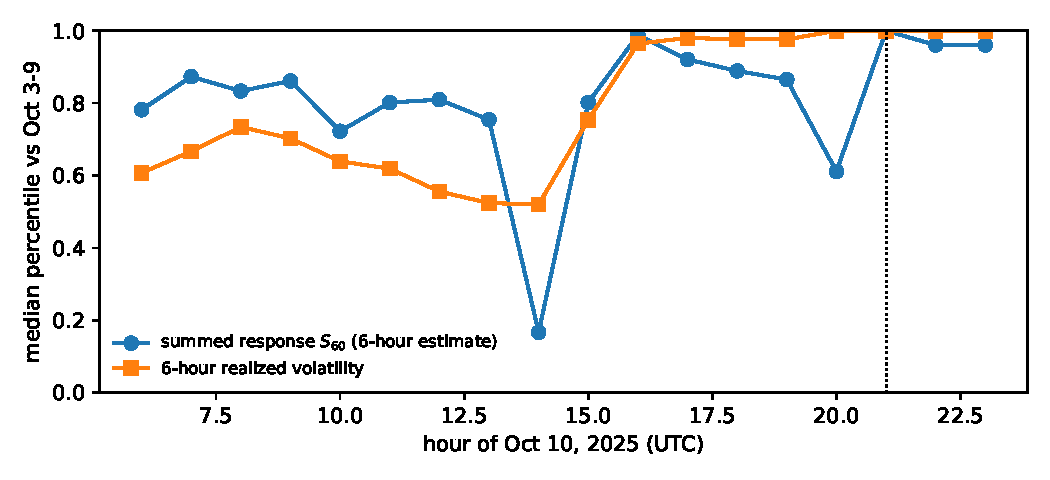
\includegraphics[width=0.72\textwidth]{figs/fig_oct10.pdf}
\caption{October 10, 2025: median percentile, across thin symbols, of the six-hour summed response $S_{60}$ and of six-hour realized volatility, relative to each symbol's October 3--9 distribution. Dotted line: the crash hour (21:00 UTC). Descriptive; the event was chosen after the fact.}\label{fig:oct10}
\end{figure}

Figure~\ref{fig:oct10} shows two things. First, the summed response was elevated through the whole day: in the morning, before volatility rose, the median thin symbol's $S_{60}$ sat at the 72nd to 87th percentile of its previous week, against the 52nd to 73rd for volatility, and at the start of the crash hour 16 of 18 thin symbols with valid estimates were above their previous-week 90th percentile. Second, volatility reached the top of its range from 16:00 onward as well, so on this day the summed response did not warn of anything volatility missed in the final hours; and across symbols it did not rank which coins fell furthest (Spearman $-0.11$, against $+0.36$ for volatility). We draw no inference from one day. The episode is consistent with the thin-book result, an elevated dynamic risk state that sizes excursions rather than timing them, and it illustrates why the paper's claims are about the size of the next hour's excursion, not about predicting crashes.

\subsection{Every pre-registered test}\label{sec:alltests}
Table~\ref{tab:alltests} lists every pre-registered test in this paper, with its outcome and the number of times its test set was opened. Of twenty-five pre-registered primaries, fifteen pass, nine fail and one was not tested because the test it depended on failed. The failures are in BTCUSDT futures, in BTCUSDT spot, on Bybit with trades alone, on Coinbase (Part 17), in the six-hour position-sizing backtest, in the two five-minute open-interest liquidation-mechanism primaries (Part 22), in the unbounded-rescaling 18-hour matched-breach capacity test (Part 23), and in the strict joint placebo clause of the persistence mediation test (Part 25, where 15-minute persistence mediates $97.6\%$ of $\hat C_3$'s excursion $\Delta R^2$ while the five-minute jump placebo also exceeds $50\%$). Five forecasting passes are in thin Binance books (including 15-minute persistence in Part 25), one in thin US stocks, two on untouched days (Part 15), three on untouched symbols (Part 16), and two in the capped Rule 15c3-5 pre-trade throttle test (Part 24); the certified-guard backtest passes narrowly; and the Bybit test with depth meets its criterion with a negligible effect. The analyses of Parts 19--21 (Section~\ref{sec:p1921}) were specified in advance but not hash-registered and are not counted here. Figure~\ref{fig:forest} adds the post-hoc checks.

\begin{table}[!htbp]\centering\footnotesize\renewcommand{\arraystretch}{0.80}\setlength{\abovecaptionskip}{3pt}
\begin{threeparttable}
\caption{All pre-registered tests}\label{tab:alltests}
\setlength{\tabcolsep}{3pt}
\begin{tabular}{p{0.31\textwidth}lp{0.27\textwidth}cc}
\toprule
Test (specification hash) & Sample & Primary statistic [CI] & Result & Opened\\
\midrule
BTCUSDT futures, MAE $\mid\hat C_3$ (\texttt{d9521218}) & 2025--26 & $\Delta R^2$ $+0.018$ [$-0.100$, $+0.132$] & fail & 1\\
BTCUSDT spot, MAE $\mid$ amplification (\texttt{b1fd7f8e}) & 2024 & $\Delta R^2$ $-0.023$ [$-0.056$, $-0.002$] & fail & 3\\
Thin books, 10 symbols (\texttt{5910b6b4}) & 2025--26 & $\Delta R^2$ $+1.216$ [$+0.273$, $+7.987$] & pass & 2\\
New thin symbols, 10 (\texttt{6aa8e2c0}) & 2025--26 & $\Delta R^2$ $+0.845$ [$+0.303$, $+6.371$] & pass & 1\\
Fresh days, 20 thin, impact controls (\texttt{65acda36}) & 2025--26 & $\Delta R^2$ $+1.583$ [$+0.588$, $+3.237$] & pass & 1\\
Position sizing, same specification & 2025--26 & $\Delta\log{\rm TLR}$ $-0.017$ [$-0.045$, $+0.011$] & fail & 1\\
Bybit, 14 coins, depth-free & 2025--26 & $\Delta R^2$ $-0.000$ [$-0.001$, $+0.001$] & fail & 1\\
Beyond volatility forecasting, 20 thin (\texttt{71983f1a}) & 2025--26 & $\Delta R^2$ $+2.787$ [$+1.425$, $+4.944$] & pass & 1\\
Certified guard, position sizing (\texttt{b9a56af4}) & 2025--26 & $\Delta\log{\rm TLR}$ $-0.024$ [$-0.051$, $-0.0004$] & pass & 1\\
Bybit with order-book depth, 6 coins (\texttt{ec2145fa}) & 2025--26 & $\Delta R^2$ $+0.033$ [$+0.019$, $+0.053$] & pass & 1\\
Thin US stocks, 23, depth-free (\texttt{f5800a69}) & 2025--26 & $\Delta R^2$ $+0.499$ [$+0.272$, $+0.779$] & pass & 1\\
Untouched days, frozen model (\texttt{69849c96}) & 2025--26 & $\Delta R^2$ $+4.196$ [$+1.551$, $+8.233$] & pass & 1\\
Untouched days, guard vs static (same) & 2025--26 & $\Delta\log{\rm TLR}$ $-0.084$ [$-0.173$, $-0.011$] & pass & 1\\
Untouched symbols, 5 thin (\texttt{0523e476}) & 2025--26 & $\Delta R^2$ $+0.727$ [$+0.377$, $+1.428$] & pass & 1\\
Untouched symbols, beyond VPIN (same) & 2025--26 & $\Delta R^2$ $+0.562$ [$+0.274$, $+1.159$] & pass & 1\\
Untouched symbols, guard vs static (same) & 2025--26 & $\Delta\log{\rm TLR}$ $-0.256$ [$-0.497$, $-0.021$] & pass & 1\\
New venue, Coinbase, 6 thin (\texttt{3233c52b}) & 2025--26 & $\Delta R^2$ $-0.092$ [$-0.407$, $+0.158$] & fail & 1\\
Coinbase, real minus placebo (same) & 2025--26 & $+0.013$ [$-0.331$, $+0.298$] & not tested & 1\\
OI liquidation forecast, 19 thin (\texttt{2b3794e3}) & 2025--26 & $\Delta R^2_{\rm LIQ}$ $-0.795$ [$-1.529$, $-0.179$] & fail & 1\\
OI liquidation mediation, 19 thin (same) & 2025--26 & Share $-6.8\%$ [$-10.2\%$, $-3.1\%$] & fail & 1\\
Non-resetting 18h guard capacity (\texttt{d4169377}) & 2025--26 & $\Delta\overline{N}$ (k\$) $+332.8$ [$-20.4$, $+1180.8$] & fail & 1\\
Capped 18h throttle liq.\ rate (\texttt{698f9119}) & 2025--26 & $\Delta{\rm Liq}$ $-7.41$ [$-11.45$, $-4.15$] pp & pass & 1\\
Capped 18h throttle ES$_{95}$ (same) & 2025--26 & $\Delta{\rm ES}_{95}$ (k\$) $-26.4$ [$-53.1$, $-6.3$] & pass & 1\\
Persistence forecast, 19 thin (\texttt{8ebd67f3}) & 2025--26 & $\Delta R^2_{\rm pers}$ $+3.713$ [$+1.884$, $+6.035$] & pass & 1\\
Persistence mediation + placebo (same) & 2025--26 & Share $97.6\%$ [$96.6\%$, $98.3\%$] & fail & 1\\
\bottomrule
\end{tabular}
\begin{tablenotes}\scriptsize\item $\Delta R^2$ in percentage points. ``Opened'' counts executions of the test cell; the repeated openings used unchanged code and specifications (Sections~\ref{sec:x6} and~\ref{sec:spot}). Intervals are 95\%, except 97.5\% for the two fresh-day primaries and the two Part 15 primaries. \end{tablenotes}
\end{threeparttable}
\end{table}

\begin{figure}[p]\centering
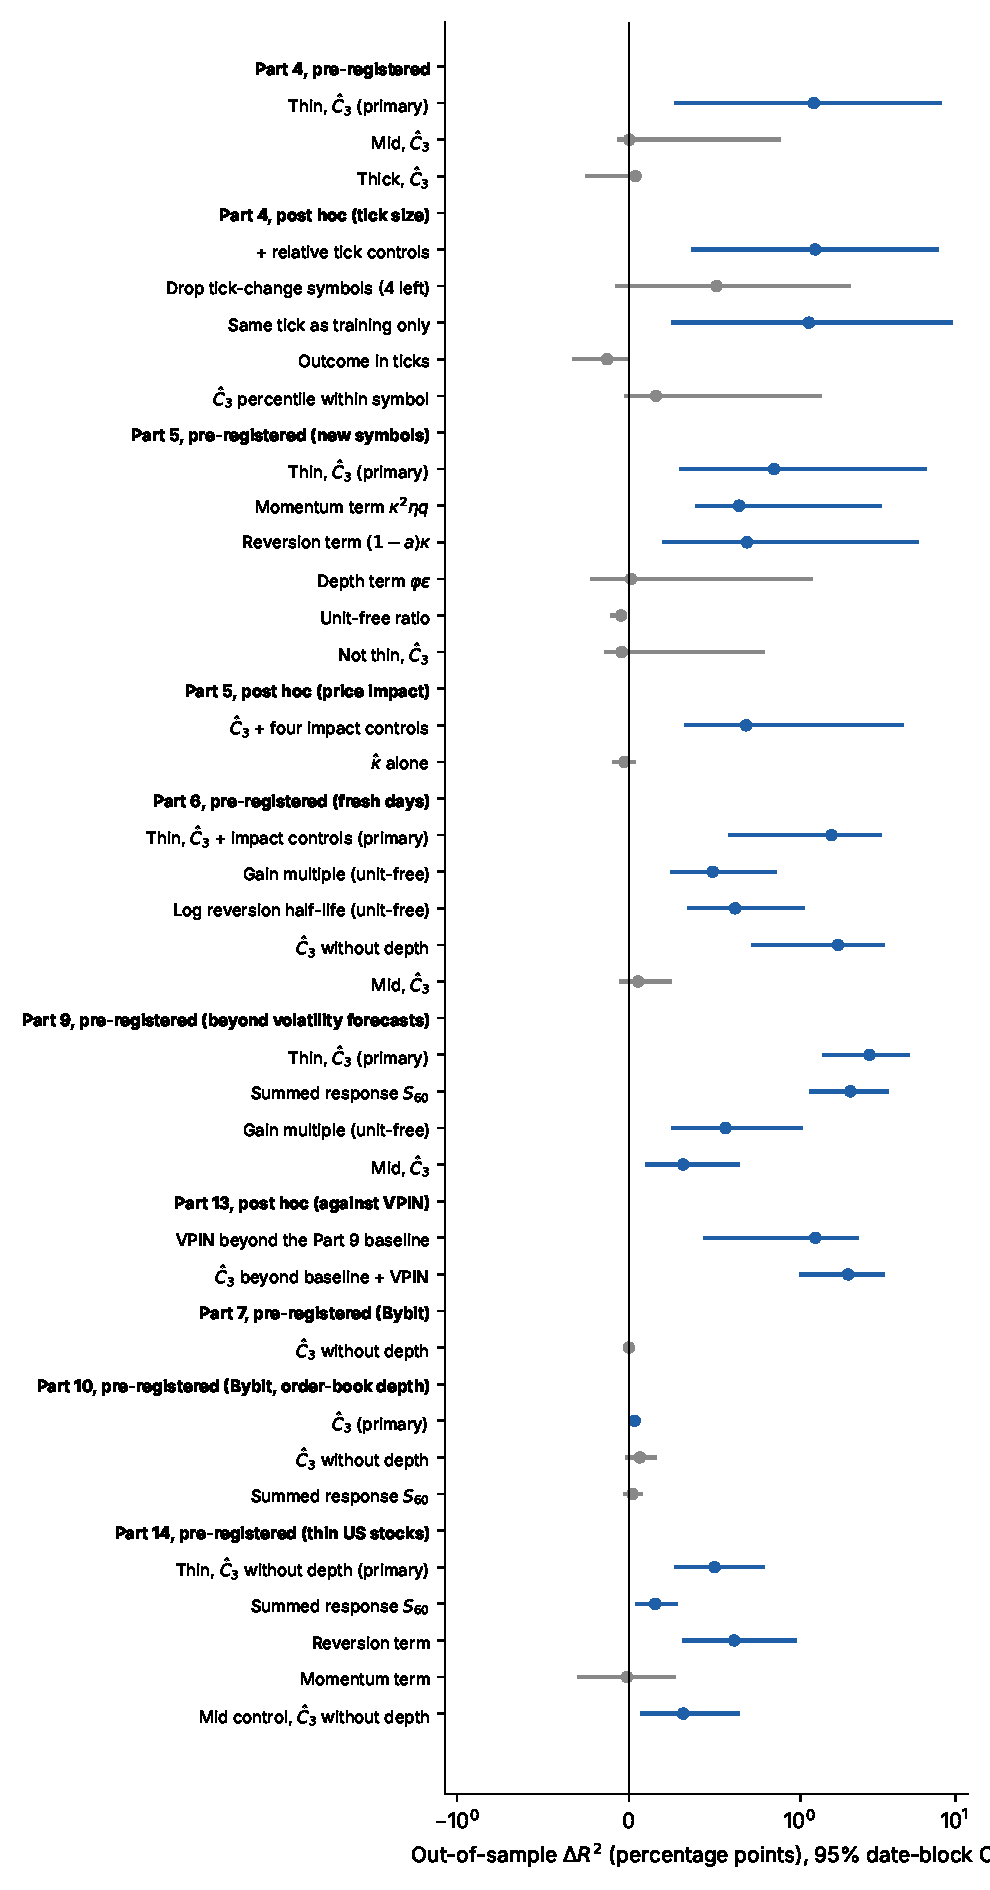
\includegraphics[height=0.82\textheight,width=0.98\textwidth,keepaspectratio]{figs/fig_forest.pdf}
\caption{Every out-of-sample forecasting evaluation in this paper's thin-book program. Points are $\Delta R^2$ in percentage points with date-block bootstrap intervals (symmetric-log axis). Blue: interval above zero. Pre-registered and post-hoc evaluations are grouped separately.}\label{fig:forest}
\end{figure}

\subsection{Threats to validity}\label{sec:threats}
\paragraph{Multiple testing.} The program registered twenty-five primaries, of which twenty-four were tested, and ran the post-hoc checks of Figure~\ref{fig:forest}. The ten passing forecasting primaries have Clark--West statistics between $5.0$ and $14.8$ (one-sided $p<0.001$ in each), the Part 15 guard primary has a one-sided bootstrap $p$ of $0.0025$, and the two Part 24 capped-throttle primaries have one-sided bootstrap $p\le 0.002$; the nine failures are reported with the same prominence.

\paragraph{Sequential design.} The program was sequential. Each pre-registration fixed one test's specification before its test data were opened, but which test to run next was chosen after the earlier results were known: new symbols after the first pass, impact controls and then a volatility baseline in response to the obvious objections, depth on Bybit after the trade-only test failed, a regulated market after the second venue gave a negligible effect, untouched days and symbols after the information-safety theory, and a certified operator after the six-hour backtest failed, and a new venue last. Pre-registration therefore protects each test from specification search on its own test data; it does not protect the program from choices that adapted across tests. That is why every test is reported, failures included (Figure~\ref{fig:forest}), and why the correction above is taken over all tested primaries.

\paragraph{Dependence among the passes.} The four passing tests share the 2023--2024 training days, and the original ten thin symbols appear in three of them. They are not four independent replications. They vary three things one at a time: the symbols (Table~\ref{tab:y6}, ten new symbols), the test days (Tables~\ref{tab:z6} and~\ref{tab:z9}, days never used before) and the baseline (impact controls, then a full volatility-forecasting model). The Part 16 test (Table~\ref{tab:p16}) shares their training days but none of their symbols. The US test (Table~\ref{tab:us}) shares none of their data: a different market, asset class, data source, universe and set of days.

\paragraph{Look-ahead and estimated regressors.} Every feature uses minutes before the forecast hour; winsorization limits, flow scales, $\theta$ and tail thresholds come from training data; and a scrambling audit leaves every hourly feature unchanged when data from $t$ onward are permuted. $\hat C_3$ and $S_{60}$ are estimated from six hours, but the evaluation compares out-of-sample forecasts rather than testing a coefficient, so estimation error in the regressor can only attenuate the measured gain.

\paragraph{Simultaneity.} The structural fits regress the price change on same-minute flow, so $\hat\kappa$ and the depletion slope mix impact with any within-minute response of flow to price. The guard's identification results (Proposition~\ref{prop:invariance} and Theorem~\ref{thm:certcost}) concern the impulse response, not these regression coefficients, and the forecasting evidence uses $\hat C_3$ as an index whose value is judged out of sample, not as a causal parameter. Simultaneity therefore changes what $\hat C_3$ measures, not whether the out-of-sample gains are real. We tried to separate the two after the fact by instrumenting this minute's flow with last minute's flow (Part 13, \texttt{R4}), but at the one-minute scale normalized flow is almost serially uncorrelated (median first-stage correlation $0.005$), so the instrument is weak and the instrumented statistic is noise (it adds $0.01$ points of $R^2$, interval including zero). The causal content of $\hat\kappa$ therefore remains open; a convincing instrument would need order-level data.

\paragraph{Selection and survivorship.} The 30 symbols were fixed from one 2024 training day before any T6 statistic was computed, and the new symbols were drawn by a seeded procedure. Symbols had to be listed through 2026, so coins delisted after a collapse are excluded; if anything this removes the episodes in which thin-book risk was largest.

\paragraph{Economic size.} The largest gain, $2.8$ points of $R^2$ on a baseline of $18.6\%$, is a 15\% increase in the explained variance of the next hour's adverse excursion, and tail classification improves by $0.005$ of AUC. In basis points, on the test hours of Table~\ref{tab:z9} and with quintile breakpoints from training data: within each quintile of the volatility forecast, hours in the top quintile of $\hat C_3$ have a next-hour adverse excursion $25.6$ basis points larger than hours in the bottom quintile (date-block 95\% interval $[18.6,32.8]$), against a mean excursion of $112.5$ basis points, and $61$ basis points larger in the most volatile quintile; the share of hours beyond the training 95th percentile rises from $2.3\%$ in the bottom $\hat C_3$ quintile to $5.1\%$ in the top. Unconditional sorts on $S_{60}$ show no pattern; its content appears only with the controls. As a sizing input the gain is worth about a 2.4\% reduction in tail loss per unit of position once the operator is certified (Table~\ref{tab:certguard}). These are modest gains on top of a strong baseline, not a new predictor that replaces volatility.

\paragraph{In margin terms.} To express the 25.6 basis points in the units a risk manager uses, we fit a lognormal distribution to the excursions in each $\hat C_3$ quintile from its mean and median; at one common threshold the fit reproduces the observed share of hours beyond the training 95th percentile in every quintile to within 0.6 percentage points. Shifting the bottom-quintile distribution up by 25.6 basis points, the effect at a given volatility forecast, roughly doubles the probability that a $20\times$ position (liquidated after a 4\% adverse move, with 1\% maintenance margin) is liquidated within the hour, from 1.3\% to 2.7\% (2.3\% to 3.2\% across the interval for the effect). For a $10\times$ position, liquidated after 9\%, the probability almost triples, from 0.04\% to 0.11\%. On \$1M of notional at $20\times$, the extra expected loss of margin is about \$710 per hour held (\$490 to \$960; \texttt{recompute\_dollar.py}). These figures come from a fitted distribution, not a test, and they treat the hour's excursion from its opening price as the liquidation trigger. They show that a difference that is small in basis points is large in the tail that leverage makes relevant, which is where a pre-trade control operates.

\paragraph{Venue.} The size of the result depends on the venue. It is largest in thin Binance USD-M books; in thin US stocks it passes a pre-registered test at about a fifth of that size, and it also appears in mid-size US stocks (Table~\ref{tab:us}); on Bybit it failed with trade data alone and, with order-book depth, met its pre-registered criterion with an effect about one eightieth of Binance's (Table~\ref{tab:bybitob}).

\subsection{What the evidence says}\label{sec:thin_summary}
Deep books sit on the stable side of the amplification condition. Flow depletes the side it hits on a fixed price grid, although re-centred depth bands make it look like replenishment, and we observe no peak overshoot. In thin Binance books the condition is still negative on average but binds more often, and the six-hour estimates of cumulative transient risk forecast the size of the next hour's adverse excursion out of sample. Four pre-registered tests pass, on the original symbols, on ten new symbols, on fresh days with price-impact controls, and on fresh days beyond a full volatility-forecasting baseline, where the gain is largest ($+2.8$ points of $R^2$) and extends to tail classification. The summed response $S$ of Theorem~\ref{thm:sum}, the guard's own statistic, carries the same information, and unit-free versions work. The content does not run through depth depletion, and in Binance books it is much weaker at mid depth and absent in BTCUSDT. In thin US stocks a fifth pre-registered forecasting test passes, at about a fifth of the Binance size and with a gain in mid-size stocks too; on Bybit the statistic is absent with trades alone and negligible with depth; and as a position-sizing input it improves a volatility limit only modestly once the operator is certified. Thin books are risky because their prices revert too slowly relative to the impact and momentum of the flow that moves them, which is what $S=\tilde\kappa/(m-q\tilde\kappa)$ measures.
